Bevor genauer in die Arbeit eingestiegen werden kann, müssen jedoch zunächst erst einmal ein paar Begriffe geklärt, die Ausgangssituation dargestellt und das Thema etwas abgesteckt werden.

\section{Begriffe}
Im folgenden sollen erst ein paar Begriffe geklärt werden, die in dieser Arbeit öfters vorkommen.
\subsubsection{App/Applikation/Anwendung}
Wenn in dieser Arbeit von einer App oder Applikation geredet wird, so ist hiermit eine Anwendung gemeint, die für mobile Endgeräte, vor allem Smartphones mit den Betriebssystemen Android beziehungsweise iOS gebaut wurden.
\subsubsection{Multi-Plattform-Anwendung}
Außerdem ist in dieser Arbeit oft die Rede von Multi-Plattform-Anwendungen. Darunter versteht man eine Anwendung, die nicht nur für eine Plattform geschrieben wurde, sondern für mehrere. Dies beinhaltet dann beispielsweise die verschiedenen Smartphone Plattformen, oder aber auch die verschiedenen PC Plattformen wie Linux oder MacOS. Eine Anwendung muss dabei auch nicht alle Plattformen beinhalten, sonder kann auch nur zwei abdecken. 
\subsubsection{Cross-Plattform-Anwendung}
Ein weiterer Begriff der in der Arbeit häufig fallen wird ist Cross-Plattform-Anwendungen. Es sind Anwendungen, die nicht nur für eine Plattform geschrieben wurde, sondern für mehrere. Auf den ersten Eindruck also exakt das gleiche wie Multi-Plattform. Jedoch ist die Besonderheit, dass bei Cross-Plattform Anwendungen, der Code nur einmal geschrieben wurde. Beide Begriffe beinhalten also erst mal, dass es eine Anwendung für mehrere Plattformen ist, mit dem Unterschied dass bei Multi-Plattform Anwendungen auch mehrere Programmiersprachen und Quellcodes erzeugt werden können, während bei Cross-Plattform nur ein Quellcode für alle geschrieben wird.


\section{Projektbeschreibung}
Als Basis für diese Arbeit wird eine bereits bestehende Elixir-Web-Anwendung genutzt. Hierbei handelt  es sich um eine Plattform, die das Ziel hat, das Verleihen und Leihen innerhalb von Bekanntschaftskreisen zu vereinfachen/ ermöglichen. Hierfür kann jeder Nutzer seine eigenen, verleihbaren Gegenstände auf der Plattform eintragen. Zusätzlich können Nutzer sogenannte Kreise erstellen und zusammen mit Freunden bzw. Familie beitreten. Jeder kann dann die Gegenstände sehen, die in den verschiedenen Kreisen vorhanden sind, in denen er Mitglied ist. Zur Kontaktaufnahme gibt es ein Chatsystem, bei dem sich Leute Nachrichten hin und her schicken können, um den Austausch zu organisieren.

\section{Funktionsumfang der Beispiel Anwendung}
Grundsätzlich wurde beim Entwurf des Funktionsumfang versucht, die typischen Funktionalitäten von Applikationen abzubilden. Eine Befragung mobiler Anwendungsentwickler durch JetBrains ergab, dass die wichtigsten Funktionen Datenspeicherung, Kommunikation über Netzwerk, Medienanzeige, Status und Navigationsmanagment, Datensynchronisierung, Dateien lesen/schreiben, Sicherheit, Bezahlung, Berechnungen und Machine Learning sind\cite{JetBrains_miscellaneous_2021}. Natürlich sind gerade der letzte Punkt oder die Bezahlung eine sehr Anwendungsfallspezifische Sache, jedoch gibt es einem einen guten Kompass was eine App so grundlegend Abzudecken hat.
Um den Arbeitsaufwand realistisch zu halten und trotzdem aber einige der oben genannten Parameter abzudecken, ist die Implementierung wie im Folgenden beschrieben eingeschränkt:

Allgemein soll eine App gebaut werden, die wie bereits erwähnt sich an einer bestehende Webanwendung orientiert und einen Teil der Funktionalität durch die Programmierung abbilden soll. Des weiteren wird eine GraphQL-Schnittstelle genutzt um die Daten der Webanwendung zu Nutzen. 

\subsection{Nativer und Cross-Plattform Ansatz}
Bei der Nativen und der Multi-Plattform Applikation bilden wir den in Abbildung \ref{fig:pageflow} dargestellten Ablauf ab. Dabei sind diese komplett durch in der Applikation implementierten Seiten dargestellt. Diese sind eine Startseite, eine Login- , Profil- , Kommunikations- und einer Chatseite. Dadurch schaffen wir es, die oben genannte Aspekte bis auf Bezahlung und Machine Learning, die für diese Applikation auch kein Anwendungsfall haben, größtenteils abzudecken. Denn durch den Login etwa erfüllt die Applikation teilweise die Bereiche Sicherheit, Statusmanagment, Daten lesen/schreiben und Kommunikation über Netzwerk. 

\begin{figure}[ht]
  \centering
  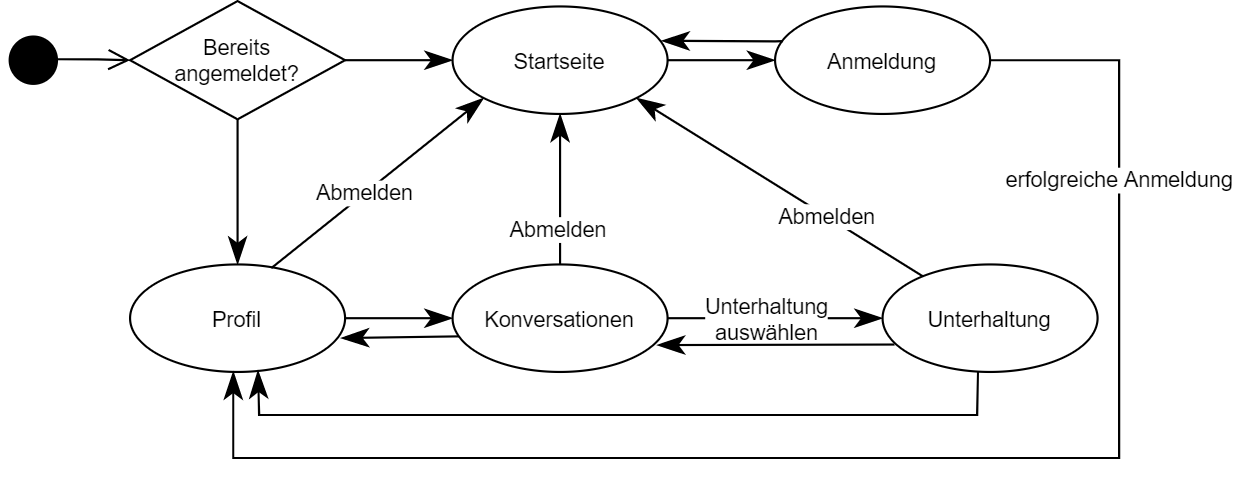
\includegraphics[height=7cm,keepaspectratio]{images/Pageflow_native_flutter.png} 
  \caption{Verbindungen zwischen den Seiten der implementierten Applikation beim nativen Ansatz und dem Multi-Plattform-Ansatz}
  \label{fig:pageflow}
\end{figure}

Der genaue Ablauf der App ist, dass der Nutzer die App öffnet. Ist er bereits eingeloggt, wird er automatisch auf die Profil Seite übergeleitet, auf der seine eigenen Sachen angezeigt werden. Ist er nicht angemeldet, so landet er auf einer Startseite/ Willkommensseite, auf der einige Sachen über das Projekt erklärt werden und kann dann zu der Loginseite weiter, von der er nach erfolgreichem Anmelden zu der bereits erwähnten Profilseite kommt. Über einen Knopf in der Menüleiste der App kann der eingeloggte Nutzer auf die Konversationsseite wechseln. Hier wird im eine Liste an Konversationen angezeigt, an denen er beteiligt ist. Nun kann er durch einen Klick auf eine Unterhaltung zu dem Chat wechseln, kann hier die bereits bestehenden Nachrichten lesen und neue Nachrichten abschicken. Mit der Zurück-Taste kann er dann wieder zu der Konversationsseite zurückkehren oder über einen Klick auf das Logo zur Profilseite zurückkehren. Als letztes ist in der Menüleiste noch ein Knopf mit dem Text "Abmelden". Wenn man diesen drückt, werden die gespeicherten Zugangsdaten gelöscht und der Nutzer somit abgemeldet. Nach erfolgreichem Abmelden wird er dann wieder zu der Startseite zurückgeführt.

\subsection{Hybrider und Gemischter Ansatz}
Bei den hybriden Absätzen wird die Website mit in die Applikation eingebunden. Je nach Art des hybriden Ansatzes unterscheidet sich hier der Umfang und Ablauf. So wird etwa bei den in Kapitel 4.2 vorgestellten Implementierungen unter Umständen nur die Website in einer Applikation angezeigt. In Kapitel 4.4 jedoch wird die oben erklärte Implementierung mit einer Anzeige der Website gemischt. So wird im vergleich zu Abbildung \ref{fig:pageflow} die Startseite durch die Startseite der Webseite ersetzt. Zusätzlich dazu wird durch eine veränderte Navigation über ein Seitenmenü die zusätzliche durch die Webanwendung verfügbare Funktionalität durch Verlinkung hinzugefügt. Etwa kommen hierdurch eine Übersicht der Kreise in denen der Nutzer Mitglied ist oder eine Liste der Gegenstände die man ausleihen kann hinzu.

\section{Themenabgrenzung}
In der Arbeit werden die Implementierungen auf eine Android Implementierung beschränkt, insofern sie nicht durch das Framework automatisch mit erzeugt werden. 
Das hat zwei Hauptgründe. Einerseits um den Aufwand für die Implementierung zu beschränken und andererseits sind iOS und Android insofern vergleichbar, da beide nativ auf die vollständigen Funktionalitäten der Betriebssysteme zugreifen. Außerdem sind es nicht die verschiedenen Programmiersprachen und ihre Kleinigkeiten die entscheidend sind, um native Apps zu entwickeln, sondern die Konzepte. So sagen Goadrich et Al in einer Untersuchung, welche Plattform für einen Universitätskurs passend wäre, dass etwa beide Umgebungen fähig sind sowohl 2D als auch 3D Graphiken mit OpenGL und Datenbanken und ihr Managment mit SQLite zu erzeugen \cite{iOSvsAndroid}. Weiter sagten sie, dass Studenten praktische Beispiele von integrierten Betriebssystem sehen könnten und lernen würden mit Threading, Synchronisierung und Locking umzugehen\cite{iOSvsAndroid}. Sie kommen am Ende auf den Schluss, dass es wegen diesem und anderem, kein Unterschied macht welche Plattformumgebung genau gelehrt wird und dass eine Programmierung, mit egal welchem, helfen würde, die Grundideen der mobilen Programmierung zu vermitteln \cite{iOSvsAndroid}.
Natürlich gibt es kleinere und größere Unterschiede zwischen den Programmiersprachen und der Implementierung auf den Plattformen, aber die Nutzung der Betriebssystemspezifischen Schnittstellen und die dahinter liegen Konzepte sind grundlegend gleich.
\TODO{Kein wörtliches Zitat. Übersetzt und nur Sinn mäßig und Ende vervollständigen}

Des weiteren wird in dieser Arbeit die Spieleimplementierung nicht betrachtet. Diese stellen zwar einen signifikanten Teil der in den Appstores vorhandenen Anwendungen dar, jedoch sind dies keine typischen Apps die von Appagenturen oder privaten Entwicklern produziert werden, sondern eher von Unternehmen mit Grafik- oder Spieleentwicklungshintergrund. Außerdem werden die meisten Apps nicht in Kotlin oder Swift direkt entwickelt, sondern mit Game- und Grafikprogrammen wie Unity oder ähnlichem gebaut. 

Der Schwerpunkt der Arbeit liegt außerdem auf Smartphone-Applikationen. Zwar sind in der Klasse der mobilen Endgeräte auch Laptops mit den Betriebssystemen Windows, MacOS oder die verschiedenen Linux distributionen, dennoch werden Applikationen primär für den Smartphone Markt entwickelt, während für mobile Rechner dann eher ein Programm schreibt.
\TODO{Warum auf Smartphone bei Untersuchung beschränkt?}

\section{Die verschiedenen Appentwicklungs Framework Klassen}
Wenn man über Applikationsentwicklung für mobile Endgerät spricht, wird zwischen verschiedenen Varianten unterschieden. Im Folgenden werden deshalb die verschiedenen Klassen vorgestellt und einige Vor und Nachteile genannt.
\subsection{Native Applikationen}
Native Applikationen werden entwickelt, um auf einer bestimmten Plattform, abhängig des Gerätetyps, des Betriebssystems und der Version, zu laufen. Der Quellcode wird dafür zu ausführbaren Code übersetzt \cite{IEEE_development_classes}.
Die Programmierung wird dabei in einer für die Plattform typischen Sprache geschrieben und ist dadurch nur für eine Plattform nutzbar. Es gibt folglich für jede Plattform einen eigenen Quellcode. Um etwa eine native Android App zu entwickeln, wird diese in Kotlin programmiert und im Anschluss in Kotlin-Bytecode übersetzt. Dieser Bytecode ist dann nur auf einem Android Gerät ausführbar.

Der Vorteil der nativen Entwicklung ist, dass man die Funktionen der verschiedenen Plattform optimal nutzen kann. So ist etwa eine Nutzung der Kamera, GPS, Beschleunigungssensoren, Kalender und vielem mehr sehr einfach. Es gibt eindeutig definierte Schnittstellen und diese müssen nur aufgerufen werden. Dabei ist die Ausführung nicht nur schnell, sondern kann auch einfach im Hintergrund ausgeführt werden \cite{IEEE_development_classes}. Dazu kommt, dass das Aussehen und die Benutzerschnittstellen ähnlich zu dem Gesamtsystem sind. So entsteht für den Nutzer ein geschlossenes System, das leichter zu bedienen ist, da es keine Unterschiede in Struktur, Design, Aufbau oder auch Benutzung gibt \cite{IEEE_Khackouch_Al}.

Einer der größten Nachteile der nativen Entwicklung jedoch ist der Aufwand und die damit verbundenen Kosten, um für die verschiedenen Plattformen eine Applikation anbieten zu können. Denn die Applikation muss für jede Plattform komplett neu gebaut werden. So können die Kosten für eine Plattform mit der Anzahl der abzudeckenden Plattformen multipliziert werden, um die Gesamtkosten zu erhalten \cite{IEEE_Khackouch_Al}. Doch nicht nur die Programmierung ist ein Kostenfaktor. So nennen Delia et Al. das Testen, Warten und Verteilen neuer Version als Faktoren, die auf jeder einzelnen unterstützten Plattform auftreten \cite{IEEE_development_classes}. Dazu kommt, dass man für jede Plattform auch Entwickler benötigt, da sich die wenigsten Entwickler auf allen Plattformen auskennen und Anwendungen für die verschiedenen Plattformen oft auch gleichzeitig entwickelt werden sollen. Um große Kosten zu verhindern, werden deswegen häufig nur  eine oder zwei Plattformen ausgewählt, wodurch die Reichweite der Anwendung sinkt.

\subsection{Web-Applikationen}
Web-Applikationen sind Applikationen, die im Netz verfügbar sind. Sie sind darauf ausgelegt, als Webseiten auf einem Server zu laufen und dann über den Browser der Geräte aufgerufen zu werden. Dieser Ansatz ist simpel, da eine Webseite sofort für jeden Nutzer verfügbar ist, sobald sie auf dem Server gestartet wurde. Sie muss auch nur einmal entwickelt werden, da sie auf allen Geräten mit einem Browser und einer Internetverbindung aufgerufen werden kann. So kann man alle Plattformen mit nur einer Entwicklung abdecken \cite{IEEE_development_classes}.

Wie gerade erwähnt, wird ein Code für alle Plattformen geschrieben. Dies ist natürlich ein großer Pluspunkt, falls die Entwicklungskosten stark eingeschränkt sind. Außerdem stehen dem Nutzer Updates direkt nach einem Neustart des Servers zur Verfügung, da es nicht erst an die Geräte verteilt und dann installiert werden muss \cite{IEEE_Khackouch_Al}.

Jedoch hat man hier große Einschränkungen in der Funktionalität, da lediglich die Funktionen des Browser zur Verfügung stehen. So können derartige Anwendungen die nativen Schnittstellen nicht benutzen und sind in ihrer Funktionalität stark beschränkt \cite{Phyo}. Dazu kommt, dass falls keine Internetverbindung vorhanden ist, die Anwendung gar nicht genutzt werden kann und bei einer langsamen Internetverbindung die Performance signifikant sinkt \cite{IEEE_Khackouch_Al}. Außerdem müssen Webanwendungen auch angepasst werden, um gut auf einem mobilen Endgerät genutzt werden zu können. So sind Smartphones etwa höher als sie breit sind, während Computerbildschirme breiter sind als sie hoch sind. Dementsprechend muss etwa eine Menüleiste darauf reagieren können und je nach Seitenverhältnis beziehungsweise Auflösung ein anderes Design anbieten. Dadurch muss Zeit investiert werden, um Webseiten zu entwickeln, die auf allen Geräten gut nutzbar sind.

Web-Applikationen sind gerade in den letzten Jahren durch die Verfügbarkeit von schnellen Internetverbindungen in fast allen Gebieten der Welt, immer beliebter geworden. Da der Fokus dieser Arbeit aber auf Smartphone Applikationen liegt, die tatsächlich auf dem Gerät installiert werden, wird diese Klasse nicht genauer betrachtet.

\newpage

\subsection{Hybride Applikationen}
Eine Klasse die dafür viel mit der vorherigen Klasse zu tun hat und in der Arbeit untersucht wird, sind die hybriden Apps. Diese sind Applikationen die zu einem Teil aus nativem Code bestehen und zu einem anderen Teil aus einem Web-Container in dem Inhalte aus dem Netz angezeigt werden. Sie benutzen also Web-Technologien, benutzen dabei aber nicht den Browser, sondern einen Web-Container. Unter Umständen kann dieser mit Hilfe von bestimmten API-Schnittstellen auf gerätespezifische Funktionen zugreifen \cite{IEEE_development_classes}.

njik
\TODO{So umschreiben dass Teil aus Kapitel 4 hier rein kommt.}

Grundsätzlich hat diese Klasse die gleichen Vor- und Nachteile wie die vorherige, da sie zu einem großen Teil aus einer Web-Applikation bestehen, die in einer nativen App angezeigt werden. Es gelten hier jedoch einige Ausnahmen, auf die auch noch einmal genauer in dem Kapitel mit der Implementierung zu dieser Klasse eingegangen wird. Denn je nach Art von hybrider App werden einzelne Probleme durch spezielle Implementierungen gelöst.Was jedoch immer ist, ist dass in den meisten Benutzeroberflächen weiterhin keine nativen Komponenten genutzt werden können und durch das Laden von Container und Website die Performance sinkt \cite{IEEE_development_classes}. Des weiteren kann die Anwendung auch weiterhin nicht im vollen Umfang genutzt werden, wenn keine Internetverbindung hat. Man hat allerdings auch eine extrem schnellere Entwicklungszeit bei bestehender Web-Anwendung, abhängig vom Umfang der nativen Integration.

\subsection{Cross-Plattform Applikationen}
Die letzte Klasse sind Multi-Plattform Applikationen. Sie zeichnen sich dadurch aus, dass jeweils nur ein Code geschrieben wird und am Ende eine Applikation für mehrere Plattformen entsteht. 

Sie haben den großen Vorteil, dass sie in der Entwicklung deutlich billiger sind als wenn man eine Anwendung für jede Plattform eine eigene Schreiben würde. Auch die Entwicklungszeit wird dadurch oft deutlich verkürzt. Durch die Devise, dass nur ein Code geschrieben wird, treten hier auch seltener Ungereimtheiten bei der Definition und Benutzung der Schnittstellen zu etwa einem Server. Auch Logikfehler treten wenn dann bei allen Anwendungen auf und nicht nur bei bestimmten. Dies klingt zwar im ersten Moment erstmal negativ, ist aber insofern gut, da Fehler dadurch leichter reproduzierbar sind und auch bereits beim testen sofort auffallen sollten, da man lediglich einen Code testen muss.

Nachteile die für diese Entwicklungsform sind oft Frameworkspezifisch. So ist etwa ein Problem, dass manchmal nicht alle Plattformfunktionen ohne Einschränkungen genutzt werden können. Des weiteren ist bei manchen ein Kritikpunkt, dass die UI nicht Geräte-typisch aussieht. Diese Probleme sind jedoch auch Abhängig von der Art, wie die Anwendung übersetzt wurde. Im folgenden soll deswegen in zwei Gruppen unterschieden werden.

\subsubsection{Interpretierte Cross-Plattform Anwendungen}
Bei Interpretieren Cross-Plattform Anwendungen schreibt der Entwickler einen Code, der wird dann mithilfe von nativen Code während der Laufzeit in ausführbaren Code übersetzt. Das bedeutet, dass die auf dem Gerät installierte Anwendung einen nativen Teil, oftmals Frameworkcode zum Übersetzen, und einem Cross-Plattform Teil, der Anwendungslogik, besteht \cite{IEEE_development_classes}.

Wie man bereits vermuten kann ist ein Problem dieser Klasse, dass bei der Ausführung eine Zwischenschicht vorhanden ist, die für zusätzliche Latenz der Ausführung führt.

\subsubsection{Compilierte Cross-Plattform Anwendungen}
Das Problem der zusätzlichen Latenz kann durch diese Klasse verhindert werden, weswegen auch nur diese in der Arbeit untersucht wurde. Denn bei kompilierten Cross-Plattform Anwendungen wird zwar während der Entwicklung nur ein Quellcode geschrieben, jedoch wird nach der Entwicklung eine Anwendung für jede Plattform gebaut, die nur aus nativen Teilen besteht \cite{IEEE_development_classes}.
